\chapter{Functions}\label{chap:Functions}

\section{Definition and Notation}

\begin{definition}
    A \vocab{function} $f$ is a rule or relation that assigns each and every element of $x \in X$ to one and only one element $y \in Y$. We write this as $f : X \to Y$ and read it as ``$f$ maps $x$ to $Y$''. $X$ is called the \vocab{domain} of $f$, denoted $\dom f$, while $Y$ is called the \vocab{codomain} of $f$. The elements of $y$ that get mapped to under $f$ is known as the \vocab{range} of $f$, denoted $\ran f$. Mathematically, $\ran f = \bc{f(x) \mid x \in \dom f}.$
\end{definition}

To define a function, we must state its rule and specify the domain. There are two ways to represent this: \[\underbrace{f : x \mapsto x^2 + 1}_{\text{the rule}}, \; \underbrace{x \in \RR}_{\dom f} \quad \tor \quad \underbrace{f(x) = x^2 + 1}_{\text{the rule}}, \; \underbrace{x \in \RR}_{\dom f}.\]

Note that two functions are equal if and only if they have the same rule and domain. For instance, the function $g : x \mapsto x^2 + 1$, $x \in \ZZ$ is not equal to $f$ (as defined above) since their domains are not equal ($\RR \neq \ZZ$).

Note that $f$ is not the same as $f(x)$; $f$ is a \emph{map}, while $f(x)$ is the \emph{value} that $f$ maps $x$ to.

\begin{definition}
    The \vocab{graph} of $f(x)$ is the collection of all points $(x, y)$ in the $xy$-plane such that the values $x$ and $y$ satisfy $y = f(x)$.
\end{definition}

\begin{proposition}[Vertical Line Test]
    A relation $f$ is a function if and only if every vertical line $x = k \in \dom f$ cuts the graph of $y = f(x)$ at a unique point.
\end{proposition}
\begin{proof}
    By definition, a function $f$ is a relation which maps each element in the domain to one and only one image.
\end{proof}

\section{Composite Functions}

\begin{definition}
    Let $f$ and $g$ be functions. Then the \vocab{composite function} $gf$ (also notated $g \circ f$) is defined by $gf(x) = g \circ f(x) = g(f(x))$, where the domain is implicitly understood to be $\dom f$.
\end{definition}

\begin{proposition}[Existence of Composite Function]
    The composite function $gf$ exists when $\ran f \subseteq \dom g$.
\end{proposition}
\begin{proof}
    Suppose $\ran f \not\subseteq \dom g$. Then there exists some element $y$ in $\ran f$ that is not in $\dom g$. Let the pre-image of $y$ under $f$ be $x$. Then $gf(x) = g(y)$ is undefined, whence $gf$ is not well-defined and is hence not a function.
\end{proof}

Note that in general, composition of functions is not commutative, i.e. $fg \neq gf$.

We write the composition of $f$ with itself $n$ times as $f^n(x)$. For instance, $ff(x) = f(f(x))$ can be written as $f^2(x)$. This should not be confused with $\bs{f(x)}^n$.

\section{Injective, Surjective and Bijective Functions}

\begin{definition}
    A function is \vocab{injective} (one-one) if each element in its codomain has at most one pre-image. Mathematically, for all $x_1, x_2 \in \dom f$, if $f(x_1) = f(x_2)$, then $x_1 = x_2$.
\end{definition}

\begin{example}
    The function $f : \RR \to \RR$, $f(x) = \e^x$ is injective, since $\e^{x_1} = \e^{x_2}$ implies $x_1 = x_2$. However, the function $g : \RR \to \RR$, $g(x) = x^2$ is not injective, since $g(-1) = 1 = g(1)$.
\end{example}

A non-injective function can be made injective by restricting its domain. In the preceding example, if we take the domain of $g$ to be $\RR^+$, then $g$ is injective.

\begin{proposition}[Horizontal Line Test]
    A function $f$ is injective if and only if any horizontal line $y = k \in \ran f$ cuts the graph of $y = f(x)$ at a unique point.
\end{proposition}
\begin{proof}
    We only prove the backwards case as the forwards case is trivial. Suppose $y = k$ and $y = f(x)$ intersect more than once. Then there exist two distinct elements $x_1$ and $x_2$ in $\dom f$ such that $f(x_1) = f(x_2)$, whence $f$ is not injective.
\end{proof}

\begin{proposition}[Strict Monotonicity Implies Injectivity]
    All strictly monotone functions are injective.
\end{proposition}
\begin{proof}
    Seeking a contradiction, assume that there exists a strictly increasing function $f : X \to Y$ which is not injective. Then there exists $x_1, x_2 \in X$ such that $f(x_1) = f(x_2)$ but $x_1 \neq x_2$. Without loss of generality, assume $x_1 < x_2$. But because $f$ is strictly increasing, we have $f(x_1) < f(x_2)$, a contradiction. Therefore, all strictly increasing functions are injective. Similarly, all strictly decreasing functions are injective.
\end{proof}

To prove that a function is not injective, it is sufficient to provide a specific counter-example.

\begin{definition}
    A function is \vocab{surjective} (onto) if each element in its codomain has at least one pre-image. Mathematically, for all $y \in Y$, there exists some $x \in X$ such that $y = f(x)$.
\end{definition}

Equivalently, a function is surjective if its range and codomain are equal.

\begin{example}
    The function $f : \RR \to \RR$, $f(x) = x^3$ is surjective, since for all $y \in \RR$, there exists some $x \in \RR$ such that $y = x^3$, namely $x = \sqrt[3]{x}$. However, the function $g : \RR \to \RR$, $g(x) = x^2$ is not surjective, since there is no $x \in \RR$ such that $x^2 = -1$.
\end{example}

Any function can be made surjective by restricting its codomain to be equal to its range. In the preceding example, if we instead define $g : \RR \to [0, \infty)$, $g(x) = x^2$ is surjective.

\begin{definition}
    A function is \vocab{bijective} (one-one and onto) if it is both injective and surjective. That is, each element in its codomain has a unique pre-image.
\end{definition}

\begin{example}
    Linear functions $f : \RR \to \RR$, $f(x) = ax + b$, where $a \neq 0$, are bijections.
\end{example}

Any injective function can be made bijective by restricting its codomain to be equal to its range.

\section{Inverse Functions}

\begin{definition}
    Let $f : X \to Y$ be an injective function. Its \vocab{inverse function}, $\inv f : Y \to X$ is a function that undoes the operation of $f$. Mathematically, $\inv f$ is the unique function such that $\inv f \circ f(x) = x$ for all $x \in \dom f$ and $f \circ \inv f(y) = y$ for all $y \in \ran f$.
\end{definition}

Though $\inv f f$ and $f \inv f$ have the same rule, they may have different domains. This is because $\dom {\inv f f} = \dom f$, while $\dom {f \inv f} = \dom {\inv f}$.

\begin{fact}[Properties of Inverse Function]
    \phantom{.}
    \begin{itemize}
        \item $\dom f = \ran{\inv f}$ and $\ran f = \dom{\inv f}$.
        \item The graphs of $f$ and $\inv f$ are reflections of each other in the line $y = x$.
    \end{itemize}
\end{fact}

\begin{figure}[H]\tikzsetnextfilename{361}
    \centering
    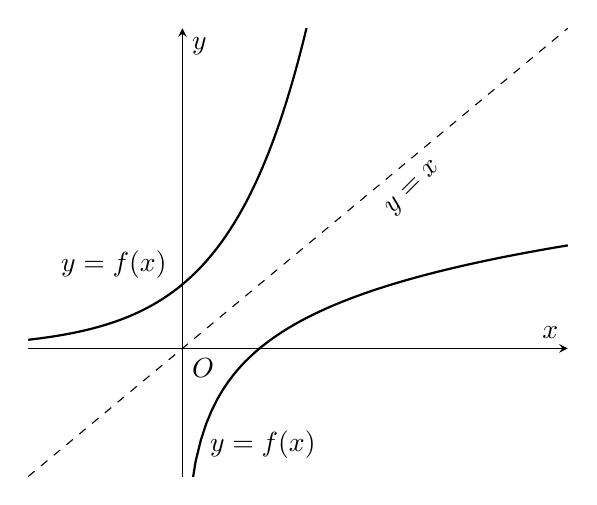
\begin{tikzpicture}
        \begin{axis}[
            domain = -2:5,
            ymin = -2,
            ymax = 5,
            samples = 101,
            axis y line=middle,
            axis x line=middle,
            xtick = \empty,
            ytick = \empty,
            xlabel = {$x$},
            ylabel = {$y$},
            legend cell align={left},
            legend pos=outer north east,
            after end axis/.code={
                \path (axis cs:0,0) 
                    node [anchor=north west] {$O$};
                }
            ]
            \addplot[thick, domain=-2:1.7] {e^x} node[pos=0.3, above left] {$y = f(x)$};
            \addplot[thick] {ln(x)} node[pos=0.25, right] {$y = \inv f(x)$};
            \addplot[dashed] {x};

            \node[rotate=45] at (3, 2.5) {$y = x$};
        \end{axis}
    \end{tikzpicture}
    \caption{The graphs of $f$ and $\inv f$ are reflections of each other in the line $y = x$.}
\end{figure}